\documentclass{standalone}
\usepackage{tikz}
\usepackage{amsmath}
\usetikzlibrary{arrows.meta, angles, quotes, calc}

\begin{document}
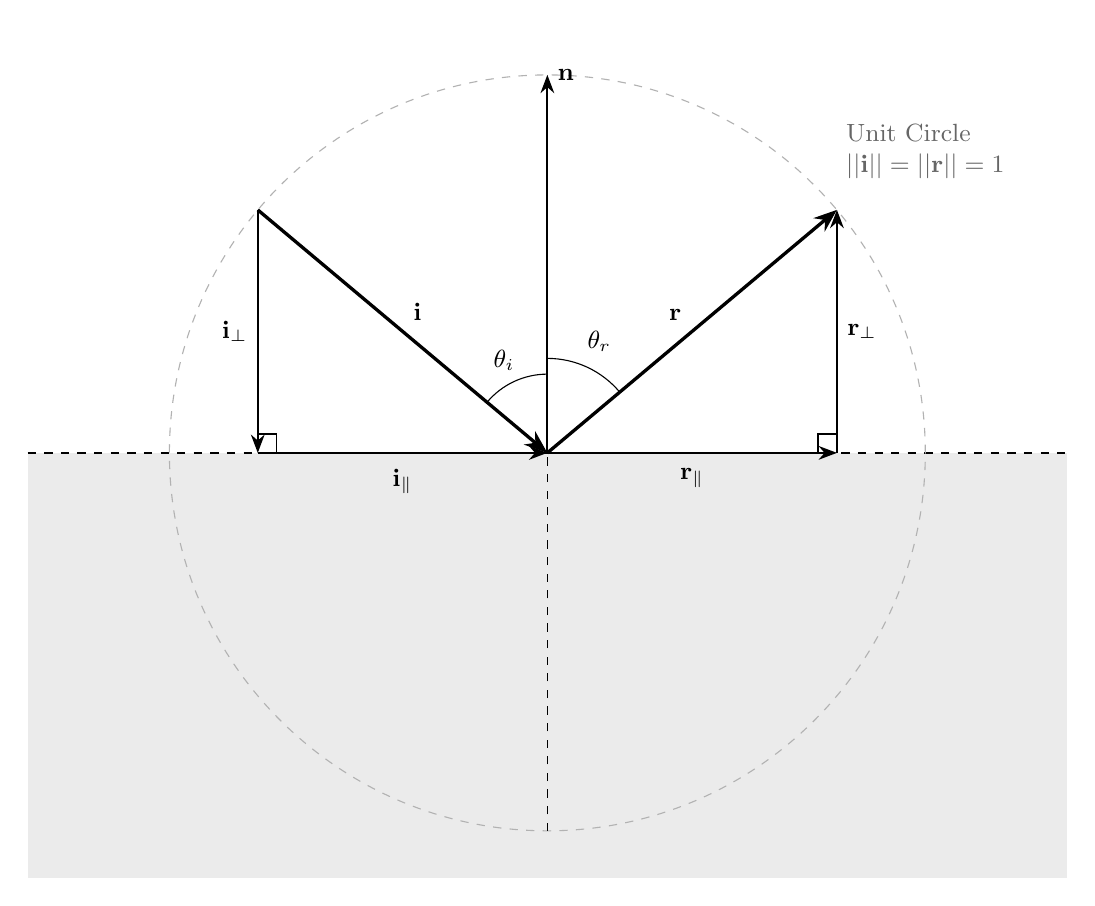
\begin{tikzpicture}[>=Stealth, font=\small, scale=1.2]
    % ================= Parameters =================
    \def\R{4}          % Unit vector radius
    \def\W{5.5}        % Half-width of canvas
    \def\H{4.5}        % Half-height (symmetric about interface y = 0)
    \def\thetaI{50}    % Angle of incidence = angle of reflection (degrees)

    % Symmetric canvas about the interface
    \path[use as bounding box] (-\W, -\H) rectangle (\W, \H);

    % Define key coordinates
    \coordinate (O) at (0,0);
    \coordinate (N_up) at (0, \R);
    \coordinate (N_down) at (0, -\R);

    % i and r vectors (Note: i points TO origin, r points FROM origin)
    \coordinate (I) at ({90+\thetaI}:\R);
    \coordinate (R) at ({90-\thetaI}:\R);

    % Projections on the interface
    \coordinate (I_x) at ({-\R*sin(\thetaI)}, 0);
    \coordinate (R_x) at ({\R*sin(\thetaI)}, 0);

    % ================= Background & Interface =================
    % Incident medium (white)
    \fill[white] (-\W, 0) rectangle (\W, \H);
    % Reflecting surface (light gray)
    \fill[black!8] (-\W, -\H) rectangle (\W, 0);

    % Interface line
    \draw[dashed, thick] (-\W, 0) -- (\W, 0);

    % ================= Unit Circle Auxiliary =================
    \draw[dashed, black!30] (O) circle (\R);
    \node[black!60, above, align=left] at (\R, 2.8) {Unit Circle\\$||\mathbf{i}|| = ||\mathbf{r}|| = 1$};

    % ================= Normal Vector =================
    \draw[dashed] (N_down) -- (O);
    \draw[->, thick] (O) -- (N_up) node[right] {$\mathbf{n}$};

    % ================= Incident Ray & Components =================
    % Components forming vector addition: i_parallel + i_perp = i
    \draw[->, thick] (I) -- (I_x) node[midway, left] {$\mathbf{i}_{\perp}$};
    \draw[->, thick] (I_x) -- (O) node[midway, below=2pt] {$\mathbf{i}_{\parallel}$};

    % Right angle symbol for incidence
    \draw (I_x) ++(0.2, 0) -- ++(0, 0.2) -- ++(-0.2, 0);

    % Main incident unit vector
    \draw[->, very thick] (I) -- (O) node[midway, above right] {$\mathbf{i}$};

    % ================= Reflected Ray & Components =================
    % Components forming vector addition: r_parallel + r_perp = r
    \draw[->, thick] (O) -- (R_x) node[midway, below=2pt] {$\mathbf{r}_{\parallel}$};
    \draw[->, thick] (R_x) -- (R) node[midway, right] {$\mathbf{r}_{\perp}$};

    % Right angle symbol for reflection
    \draw (R_x) ++(-0.2, 0) -- ++(0, 0.2) -- ++(0.2, 0);

    % Main reflected unit vector
    \draw[->, very thick] (O) -- (R) node[midway, above left] {$\mathbf{r}$};

    % ================= Angles =================
    % Angle of incidence
    \draw pic[draw, angle radius=1cm, "$\theta_i$", angle eccentricity=1.3] {angle = N_up--O--I};

    % Angle of reflection (R--O--N_up: CCW sweep matches θ_i on the right of n)
    \draw pic[draw, angle radius=1.2cm, "$\theta_r$", angle eccentricity=1.3] {angle = R--O--N_up};

\end{tikzpicture}
\end{document}
